\documentclass[10pt,a4paper]{article}

\usepackage[T1]{fontenc}
\usepackage{lmodern}
\usepackage[utf8]{inputenc}
% Polskie nazwy (Rysunek, Tabela) z pliku lokalizacji babel. Wzorców dzielenia wyrazów może nie być w instalacji.
\usepackage[english]{babel}
\babelprovide[import=pl, main]{polish}
\emergencystretch=2em
\AtBeginDocument{\renewcommand{\tablename}{Tabela}}
\usepackage[a4paper,margin=2.2cm]{geometry}
\usepackage{booktabs}
\usepackage{array}
\usepackage{xcolor}
\usepackage{amsmath,amssymb}
\usepackage{microtype}
\usepackage{caption}
\usepackage{float}
\usepackage{tikz}
\usepackage{pgfplots}
\usepgfplotslibrary{groupplots}
\usetikzlibrary{positioning,arrows.meta,calc,fit,backgrounds}
\pgfplotsset{compat=1.17}
\usepackage[hidelinks]{hyperref}

\definecolor{ctrain}{HTML}{0072B2}
\definecolor{cval}{HTML}{D55E00}
\definecolor{cscratch}{HTML}{009E73}
\definecolor{cgpt}{HTML}{7B3294}
\captionsetup{font=small,labelfont=bf}
\frenchspacing
\pgfplotsset{every axis/.append style={scaled ticks=false, /pgf/number format/use comma,
  yticklabel={\pgfmathprintnumber[fixed,fixed zerofill,precision=2,use comma]{\tick}}}}
\setlength{\parindent}{0pt}
\setlength{\parskip}{4pt}

% Miejsca do uzupełnienia.
\newcommand{\todo}[1]{\textcolor{red}{[#1]}}

\title{Klasyfikacja toksycznych komentarzy modelami decoder-only:\\
trening od zera, fine-tuning i zero-shot}
\author{Filip Pawlowicz}
\date{}

\begin{document}
\maketitle

Porównuję trzy sposoby klasyfikacji binarnej tekstu na tych samych danych i~przy tym samym limicie długości wejścia (128 tokenów): mały dekoder trenowany od zera, GPT-2 z~fine-tuningiem i~nową warstwą klasyfikacyjną oraz ten sam GPT-2 bez treningu, z~ograniczeniem wyjścia do dwóch tokenów (constrained decoding). Kod jest w~\texttt{data.ipynb} (dane, modele, eksperymenty), \texttt{train.py} (pętla treningowa, ewaluacja) i~\texttt{util.py}.

\section{Dane}

Zbiór to Jigsaw Toxic Comment Classification Challenge (Kaggle): komentarze z~dyskusji na stronach Wikipedii. Sprowadziłem zadanie do jednej etykiety binarnej \texttt{toxic}. Pozostałych pięć etykiet (\texttt{severe\_toxic}, \texttt{obscene}, \texttt{threat}, \texttt{insult}, \texttt{identity\_hate}) służy tylko do stratyfikacji podziału. Rozmiary zbiorów podaje tabela~\ref{tab:sizes}.

\begin{table}[htbp]
\centering
\begin{tabular}{lrrr}
\toprule
Zbiór & Komentarze & Toksyczne & Udział toksycznych \\
\midrule
Trening    & 143\,613 & 13\,765 & 9,58\,\% \\
Walidacja  & 15\,958  & 1\,529  & 9,58\,\% \\
Test       & 63\,978  & 6\,090  & 9,52\,\% \\
\bottomrule
\end{tabular}
\caption{Rozmiary zbiorów. Walidacja i~trening pochodzą z~\texttt{train.csv} (159\,571 komentarzy).}
\label{tab:sizes}
\end{table}

\textbf{Przetwarzanie.} Ciągi białych znaków zastępuję jedną spacją. W~zbiorze testowym zostają tylko wiersze z~jawną etykietą (etykiety z~\texttt{test\_labels.csv}, wiersze z~\texttt{toxic = -1} odpadają). Walidacja to 10\,\% zbioru treningowego, wybrane przez \texttt{MultilabelStratifiedShuffleSplit} po wszystkich sześciu etykietach (\texttt{random\_state=42}). Po tym podziale udział toksycznych w~treningu i~walidacji jest identyczny.

\textbf{Długość i~niezbalansowanie.} W~tokenach GPT-2 mediana komentarza to 48, a~90.\ percentyl to 197. Limit 128 tokenów ucina 18\,\% komentarzy (11\,\% wśród toksycznych w~treningu), a~dla tokenizera od zera 21\,\% (13\,\%). W~zero-shot prompt zabiera część tego limitu, więc na komentarz zostaje mniej tokenów: \todo{liczba tokenów promptu i~odsetek ucinanych komentarzy}. Toksycznych jest niecałe 10\,\%, więc do wyboru najlepszej epoki używam AUPRC, a~próg decyzyjny dobieram na walidacji zamiast przyjmować 0,5. Nie stosuję wag klas.

\begin{table}[htbp]
\centering
\small
\begin{tabular}{p{11.5cm}c}
\toprule
Komentarz & \texttt{toxic} \\
\midrule
You, sir, are my hero. Any chance you remember what page that's on? & 0 \\
Would you both shut up, you don't run wikipedia, especially a stupid kid. & 1 \\
\bottomrule
\end{tabular}
\caption{Przykłady ze zbioru treningowego.}
\end{table}

\section{Modele}

We wszystkich trzech podejściach wejście ma kształt $(B, T)$ ($B$ to rozmiar batcha, $T \le 128$ to liczba tokenów), padding jest po prawej, a~model zwraca jeden logit na komentarz. Strata to binarna entropia krzyżowa z~logitów, a~metryki liczy ten sam kod z~\texttt{util.py}. Klasyfikacja opiera się na stanie ostatniego tokenu wejścia (nie paddingu), bo przy masce przyczynowej to jedyna pozycja, która widziała całe wejście. W~modelu od zera i~w zero-shot indeks tego tokenu to liczba jedynek w~masce minus 1. W~GPT-2 z~warstwą klasyfikacyjną robi to biblioteka: bierze skrajnie prawy token różny od tokenu paddingu.

\subsection{Dekoder trenowany od zera}

\textbf{Tokenizer.} Własny byte-level BPE (biblioteka \texttt{tokenizers}), wytrenowany na komentarzach ze zbioru treningowego, słownik 8192 tokenów, \texttt{<|endoftext|>} jako token paddingu. Słownik GPT-2 (50\,257) przy wymiarze 128 dałby 6,4 mln parametrów w~samych embeddingach, a~zadanie dopuszcza 0,5--10 mln parametrów w~całym modelu.

\textbf{Architektura.} Dekoder w~stylu GPT: 4 bloki typu pre-LN, wymiar $d=128$, 4 głowice uwagi (po 32 wymiary), MLP z~rozszerzeniem $4d$ i~aktywacją GELU, uczone embeddingi pozycji. Dropout 0,2 działa po embeddingach, na wagach uwagi i~po projekcjach uwagi i~MLP. Warstwy liniowe w~uwadze i~MLP nie mają biasu. Wagi inicjalizuję z~$\mathcal{N}(0; 0{,}02)$, a~projekcje wyjściowe gałęzi residualnych dodatkowo skaluję przez $1/\sqrt{2L}$ ($L=4$ to liczba bloków), żeby strumień residualny nie rósł z~głębokością. Klasyfikator to MLP na stanie ostatniego tokenu: $128 \to 128$, GELU, dropout, $128 \to 1$. Nie ma głowicy modelu językowego, więc nie powstaje druga macierz $V \times d$. Parametry podaje tabela~\ref{tab:params}, a~budowę rysunek~\ref{fig:scratch}.

\begin{table}[htbp]
\centering
\begin{tabular}{lr}
\toprule
Element & Parametry \\
\midrule
Embedding tokenów ($8192 \times 128$) & 1\,048\,576 \\
Embedding pozycji ($128 \times 128$)  & 16\,384 \\
4 bloki transformera (po 197\,120)    & 788\,480 \\
LayerNorm końcowy                     & 256 \\
Klasyfikator (MLP)                    & 16\,641 \\
\midrule
Razem                                 & 1\,870\,337 \\
\bottomrule
\end{tabular}
\caption{Parametry modelu od zera (1,87 mln, plik z~wagami 7,5\,MB).}
\label{tab:params}
\end{table}

\begin{figure}[htbp]
\centering
\begin{tikzpicture}[
  box/.style={draw, rounded corners=2pt, minimum width=5.4cm, minimum height=7mm, align=center, font=\footnotesize, fill=blue!6},
  io/.style={box, fill=gray!14},
  small/.style={draw, rounded corners=2pt, minimum width=3.9cm, minimum height=6mm, align=center, font=\footnotesize, fill=blue!6},
  arr/.style={-{Stealth[length=2mm]}, thick},
  add/.style={draw, circle, inner sep=0pt, minimum size=4.5mm, font=\scriptsize, fill=white},
  node distance=5mm]
% Główny tor modelu.
\node[io] (in) {komentarz $\to$ BPE (8192), $T \le 128$ tokenów};
\node[box, below=of in] (emb) {tok\_emb $+$ pos\_emb\\ $(B,T) \to (B,T,128)$};
\node[box, below=of emb] (drop) {Dropout 0,2};
\node[box, below=of drop, fill=orange!18] (blocks) {Blok transformera $\times 4$};
\node[box, below=of blocks] (ln) {LayerNorm};
\node[box, below=of ln] (last) {stan ostatniego tokenu wejścia\\ $(B,T,128) \to (B,128)$};
\node[box, below=of last] (head) {klasyfikator: Linear $128{\to}128$, GELU,\\ Dropout, Linear $128{\to}1$};
\node[io, below=of head] (out) {logit $(B)$};
\foreach \a/\b in {in/emb, emb/drop, drop/blocks, blocks/ln, ln/last, last/head, head/out}
  \draw[arr] (\a) -- (\b);
% Szczegół bloku.
\begin{scope}[xshift=8.6cm, yshift=-1.0cm]
  \node[small] (b1) at (0,0) {LayerNorm};
  \node[small, above=6mm of b1] (b0) {wejście bloku $x$};
  \node[small, below=5mm of b1, fill=green!10] (att) {uwaga z maską przyczynową\\ 4 głowice};
  \node[add, below=5mm of att] (a1) {$+$};
  \node[small, below=5mm of a1] (b2) {LayerNorm};
  \node[small, below=5mm of b2, fill=green!10] (mlp) {MLP $128{\to}512{\to}128$\\ GELU};
  \node[add, below=5mm of mlp] (a2) {$+$};
  \node[small, below=5mm of a2] (bo) {wyjście bloku};
  \draw[arr] (b0) -- (b1);
  \draw[arr] (b1) -- (att);
  \draw[arr] (att) -- (a1);
  \draw[arr] (a1) -- (b2);
  \draw[arr] (b2) -- (mlp);
  \draw[arr] (mlp) -- (a2);
  \draw[arr] (a2) -- (bo);
  \draw[arr] ($(b0.south)+(0,-0.15)$) -- ++(2.2,0) |- (a1.east);
  \draw[arr] ($(a1.south)+(0,-0.15)$) -- ++(2.2,0) |- (a2.east);
\end{scope}
\fill ($(b0.south)+(0,-0.15)$) circle (0.6pt);
\fill ($(a1.south)+(0,-0.15)$) circle (0.6pt);
\draw[dashed, gray] (blocks.east) -- ++(0.9,0) |- (b1.west);
\node[font=\footnotesize\bfseries, above=2mm of b0] {Budowa jednego bloku};
\end{tikzpicture}
\caption{Dekoder trenowany od zera: tor główny (po lewej) i~budowa jednego bloku (po prawej). Znak $+$ w~kółku oznacza połączenie residualne. Dropout w~bloku pominięto na rysunku.}
\label{fig:scratch}
\end{figure}

\subsection{GPT-2 z~warstwą klasyfikacyjną (fine-tuning)}

Model to \texttt{gpt2} z~Hugging Face (124 mln parametrów, 12 warstw, $d=768$, 12 głowic uwagi, kontekst 1024) w~wersji \texttt{GPT2ForSequenceClassification} z~\texttt{num\_labels=1}. Biblioteka dokłada warstwę \texttt{score} ($768 \to 1$, bez biasu, 768 parametrów), której nie ma w~checkpoincie i~która startuje z~losowych wag. Tokenizer to oryginalny BPE GPT-2 (50\,257 tokenów). GPT-2 nie ma tokenu paddingu, więc używam \texttt{<|endoftext|>}, z~paddingiem po prawej. Trenuję wszystkie wagi (pełny fine-tuning, bez LoRA i~bez zamrażania warstw). Plik z~wagami ma 498\,MB, czyli 66 razy więcej niż model od zera.

\subsection{GPT-2 zero-shot z~constrained decoding}

Te same wagi wstępne i~ten sam tokenizer, ale bez treningu. Komentarz (ucięty tak, żeby całość z~promptem mieściła się w~128 tokenach) otaczam strukturą pytanie--odpowiedź. GPT-2 jest modelem bazowym, bez szablonu czatu i~bez ról, więc prompt to zwykły tekst:
\begin{center}
\texttt{Comment: <komentarz>}\\
\texttt{Question: Is the comment above toxic? Answer with Yes or No.}\\
\texttt{Answer:}
\end{center}
Prompt kończy się na \texttt{Answer:} bez spacji, bo spacja należy do tokenu odpowiedzi.
Każda klasa to grupa wariantów odpowiedzi, z~których każdy jest jednym tokenem (kod sprawdza to asercją): \texttt{" No"}, \texttt{" no"}, \texttt{" NO"} dla klasy 0 i~\texttt{" Yes"}, \texttt{" yes"}, \texttt{" YES"} dla klasy 1. Spacja jest częścią tokenu, bo odpowiedź następuje po dwukropku. Rzutuję stan ostatniego tokenu tylko na sześć odpowiadających im wierszy macierzy wyjściowej (\texttt{lm\_head}, współdzielonej z~embeddingiem tokenów), więc nie liczę logitów dla całego słownika. Logit klasy to $\ell_c = \log \sum_{w \in c} e^{\ell_w}$, a~wynikiem jest jeden logit $\ell_{\text{yes}} - \ell_{\text{no}}$. Normalizacja softmaxa po całym słowniku skraca się w~tej różnicy, więc $\sigma(\ell_{\text{yes}} - \ell_{\text{no}})$ to suma prawdopodobieństw wariantów \texttt{yes} podzielona przez sumę wariantów obu klas, a~metryki z~\texttt{util.py} działają bez zmian. Notebook zawiera test zgodności z~pełnymi logitami (na kilku przykładach). Próg dobieram na walidacji (maksimum F1 klasy toksycznej), a~nie na teście: \todo{wartość progu}.

Rozkład po dwóch grupach jest warunkowy, więc osobno mierzę, ile masy prawdopodobieństwa pełnego softmaxa przypada na tokeny obu grup i~jak często argmax w~całym słowniku jest jednym z~nich. Pomiar robię na jednym batchu walidacyjnym, żeby nie dobierać promptu na teście. Pierwsza wersja promptu (\texttt{Is the comment above toxic? Answer (yes or no):}, z~jednym tokenem na klasę) dawała na tokeny odpowiedzi średnio 8,6\,\% masy, a~najczęstszym argmaxem był znak nowej linii (76 z~128 przykładów). Dlatego przeformułowałem prompt i~zgrupowałem warianty. Do porównania liczę też masę na wszystkich wariantach, także tych spoza klas (bez spacji, inne wielkości liter): \todo{średnia masa na grupach, odsetek argmax = etykieta, masa na wariantach spoza klas}.

\begin{figure}[htbp]
\centering
\begin{tikzpicture}[
  box/.style={draw, rounded corners=2pt, minimum width=6.2cm, minimum height=7mm, align=center, font=\footnotesize, fill=blue!6},
  io/.style={box, fill=gray!14},
  arr/.style={-{Stealth[length=2mm]}, thick},
  node distance=5mm]
\node[font=\small\bfseries] (t1) at (0,0) {Fine-tuning};
\node[io, below=3mm of t1] (a0) {komentarz ($T \le 128$)};
\node[box, below=of a0, fill=orange!18] (a1) {GPT-2: 12 warstw, $d=768$\\ wszystkie wagi trenowane};
\node[box, below=of a1] (a2) {stan ostatniego tokenu wejścia\\ $h \in \mathbb{R}^{768}$};
\node[box, below=of a2, fill=green!12] (a3) {\texttt{score}: Linear $768{\to}1$ (nowa)};
\node[io, below=of a3] (a4) {logit};
\foreach \a/\b in {a0/a1, a1/a2, a2/a3, a3/a4} \draw[arr] (\a) -- (\b);

\node[font=\small\bfseries] (t2) at (6.9,0) {Zero-shot};
\node[io, below=3mm of t2] (z0) {komentarz $+$ prompt ($T \le 128$)};
\node[box, below=of z0, fill=orange!8] (z1) {GPT-2: te same wagi wstępne\\ bez treningu};
\node[box, below=of z1] (z2) {stan ostatniego tokenu wejścia\\ $h \in \mathbb{R}^{768}$};
\node[box, below=of z2, fill=green!12] (z3) {wiersze \texttt{lm\_head} dla wariantów \texttt{No}, \texttt{Yes}\\ $\ell_c = \log\sum_{w \in c} e^{\ell_w}$};
\node[io, below=of z3] (z4) {logit $= \ell_{\text{yes}} - \ell_{\text{no}}$};
\foreach \a/\b in {z0/z1, z1/z2, z2/z3, z3/z4} \draw[arr] (\a) -- (\b);
\end{tikzpicture}
\caption{Dwa sposoby użycia GPT-2. Oba kończą się jednym logitem, a~prawdopodobieństwo klasy toksycznej to $\sigma(\text{logit})$.}
\label{fig:gpt2}
\end{figure}

\section{Trening i~ewaluacja}

\subsection{Ustawienia}

Trening i~pomiary robiłem lokalnie na GeForce GTX 1660 Ti (6\,GB), z~mieszaną precyzją (fp16, \texttt{GradScaler}). Wspólne ustawienia: AdamW ($\beta=(0{,}9;\,0{,}95)$, weight decay 0,01 bez biasów i~LayerNorm), liniowa rozgrzewka przez 5\,\% kroków, potem cosinus do 10\,\% maksymalnego współczynnika uczenia (LR), przycinanie gradientu do normy 1, batch 64 w~treningu i~128 w~ewaluacji. Najlepsza epoka to ta z~najwyższym AUPRC na walidacji (poprawa mniejsza niż 0,001 się nie liczy), a~po treningu wracam do jej wag. Harmonogram LR jest liczony dla maksymalnej liczby epok, więc model od zera, zatrzymany po 8 z~10 epok, nie doszedł do końca spadku. Metryki testowe liczę z~progiem wybranym na walidacji (dla zero-shot też).

\begin{table}[htbp]
\centering
\begin{tabular}{lcc}
\toprule
 & Od zera & GPT-2 (fine-tuning) \\
\midrule
Maks.\ LR            & $5\cdot10^{-4}$ & $5\cdot10^{-5}$ \\
Maks.\ liczba epok   & 10 & 3 \\
Cierpliwość (early stopping) & 3 & 2 \\
Wykonane epoki       & 8 & 3 \\
Najlepsza epoka      & 5 & 2 \\
Próg z~walidacji     & 0,39 & 0,57 \\
\bottomrule
\end{tabular}
\caption{Hiperparametry i~przebieg treningu.}
\label{tab:setup}
\end{table}

\subsection{Krzywe uczenia}

\begin{figure}[htbp]
\centering
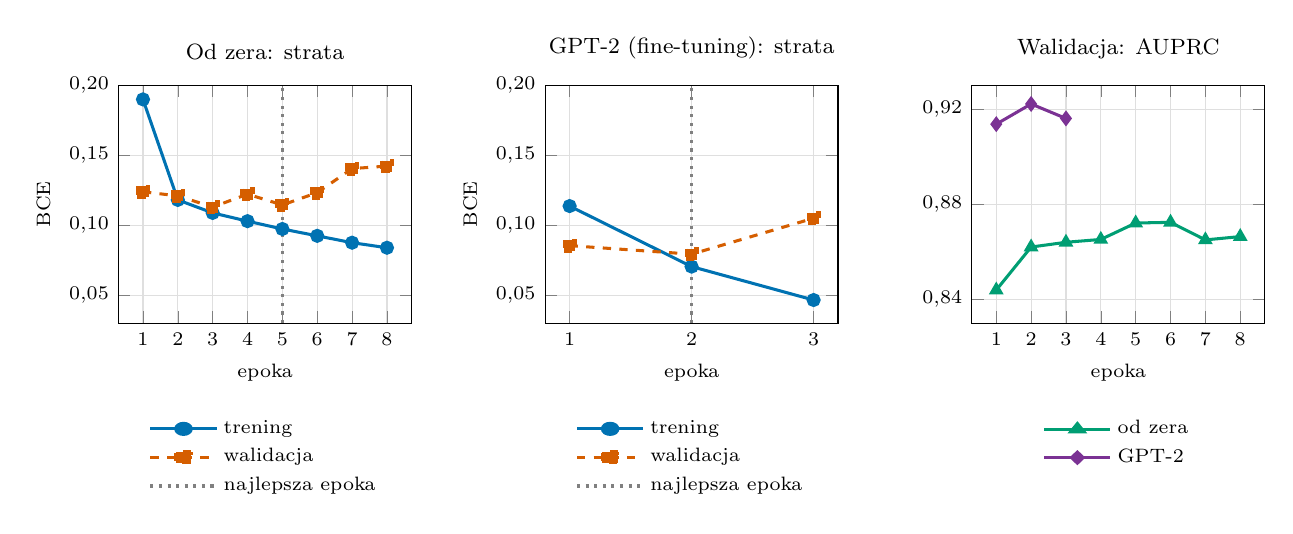
\begin{tikzpicture}
\begin{groupplot}[
  group style={group size=3 by 1, horizontal sep=1.7cm},
  width=5.3cm, height=4.6cm, grid=major, grid style={gray!25},
  every axis plot/.append style={line width=1.1pt, mark size=2pt},
  tick label style={font=\scriptsize}, label style={font=\scriptsize},
  title style={font=\footnotesize},
  legend style={font=\scriptsize, draw=none, fill=none, at={(0.5,-0.36)}, anchor=north,
    legend cell align=left},
  legend image post style={xscale=1.4},
  legend columns=1,
  xlabel={epoka}]
\nextgroupplot[title={Od zera: strata}, ylabel={BCE}, ymin=0.03, ymax=0.2, ytick={0.05,0.1,0.15,0.2},
  xtick={1,2,3,4,5,6,7,8}]
\addplot[ctrain, solid, mark=*] coordinates {(1,0.1900)(2,0.1181)(3,0.1088)(4,0.1029)(5,0.0973)(6,0.0924)(7,0.0875)(8,0.0839)};
\addplot[cval, dashed, mark=square*] coordinates {(1,0.1239)(2,0.1210)(3,0.1130)(4,0.1222)(5,0.1145)(6,0.1233)(7,0.1405)(8,0.1423)};
\addplot[gray, dotted, mark=none] coordinates {(5,0.03)(5,0.2)};
\legend{trening, walidacja, najlepsza epoka}
\nextgroupplot[title={GPT-2 (fine-tuning): strata}, ylabel={BCE}, ymin=0.03, ymax=0.2, ytick={0.05,0.1,0.15,0.2},
  xtick={1,2,3}]
\addplot[ctrain, solid, mark=*] coordinates {(1,0.1137)(2,0.0704)(3,0.0465)};
\addplot[cval, dashed, mark=square*] coordinates {(1,0.0854)(2,0.0793)(3,0.1050)};
\addplot[gray, dotted, mark=none] coordinates {(2,0.03)(2,0.2)};
\legend{trening, walidacja, najlepsza epoka}
\nextgroupplot[title={Walidacja: AUPRC}, ymin=0.83, ymax=0.93, ytick={0.84,0.88,0.92},
  xtick={1,2,3,4,5,6,7,8}]
\addplot[cscratch, solid, mark=triangle*] coordinates {(1,0.8439)(2,0.8620)(3,0.8640)(4,0.8652)(5,0.8721)(6,0.8724)(7,0.8650)(8,0.8664)};
\addplot[cgpt, solid, mark=diamond*] coordinates {(1,0.9137)(2,0.9222)(3,0.9161)};
\legend{od zera, GPT-2}
\end{groupplot}
\end{tikzpicture}
\caption{Krzywe uczenia. W panelach strat kolor oznacza zbiór (niebieski, linia ciągła, koła: trening; pomarańczowy, linia przerywana, kwadraty: walidacja). W panelu AUPRC kolor oznacza model, a pokazana jest tylko walidacja. Linia kropkowana to epoka o najwyższym AUPRC, do której wracam po treningu.}
\label{fig:curves}
\end{figure}

Rysunek~\ref{fig:curves} pokazuje przebieg treningu z~plików \texttt{history\_sc.json} i~\texttt{history\_ft.json}.

\textbf{Model od zera.} Strata treningowa spada w~każdej epoce (0,190 $\to$ 0,084), a~walidacyjna ma minimum 0,113 w~epoce 3 i~rośnie do 0,142 w~epoce 8. AUPRC na walidacji osiąga maksimum 0,872 w~epokach 5--6. Early stopping przerwał trening po epoce 8 i~przywrócił wagi z~epoki 5. Jedna epoka treningu trwa ok.\ 40\,s, cały \texttt{fit} 340\,s (z~walidacją po każdej epoce).

\textbf{GPT-2.} Strata walidacyjna jest najniższa w~epoce 2 (0,079) i~rośnie do 0,105 w~epoce 3, mimo że strata treningowa dalej spada (0,070 $\to$ 0,047). Najlepszy AUPRC na walidacji (0,922) też wypada w~epoce 2. Jedna epoka treningu trwa ok.\ 302\,s (7,5 razy dłużej niż w~modelu od zera), cały \texttt{fit} 945\,s.

\subsection{Wyniki}

Tabela~\ref{tab:results} zbiera parametry, czasy i~metryki trzech modeli.

\begin{table}[H]
\centering
\small
\setlength{\tabcolsep}{5pt}
\begin{tabular}{lccc}
\toprule
 & Od zera & GPT-2 (fine-tuning) & GPT-2 (zero-shot) \\
\midrule
Parametry                      & 1,87 mln & 124 mln & 124 mln (0 trenowanych) \\
Rozmiar pliku z~wagami         & 7,5 MB & 498 MB & --- \\
Czas treningu (cały \texttt{fit})  & 340 s & 945 s & 0 s \\
Czas jednej epoki (trening)     & ok.\ 40 s & ok.\ 302 s & --- \\
Próg decyzyjny                 & 0,39 & 0,57 & \todo{} \\
\midrule
\multicolumn{4}{l}{\textit{Walidacja (15\,958 komentarzy)}} \\
AUPRC                          & 0,872 & 0,922 & \todo{} \\
F1 (próg dobrany na tej walidacji) & 0,795 & 0,831 & \todo{} \\
\midrule
\multicolumn{4}{l}{\textit{Test (63\,978 komentarzy)}} \\
Accuracy                       & \todo{} & \todo{} & \todo{} \\
F1 klasy toksycznej            & \todo{} & \todo{} & \todo{} \\
Macro-F1                       & \todo{} & \todo{} & \todo{} \\
AUROC / AUPRC                  & \todo{} & \todo{} & \todo{} \\
Czas inferencji na teście      & \todo{} & \todo{} & \todo{} \\
\bottomrule
\end{tabular}
\caption{Porównanie modeli. Czas treningu obejmuje walidację po każdej epoce. F1 z~progiem dobranym na tym samym zbiorze jest optymistyczne. Czas inferencji obejmuje tokenizację w~\texttt{collate\_fn}.}
\label{tab:results}
\end{table}

\section{Analiza porównawcza}

\todo{Mocne i~słabe strony każdego podejścia.}

\todo{Kiedy które podejście wybrać.}

\todo{Wrażliwość na rozmiar modelu i~danych.}

\begin{thebibliography}{9}\small
\item A.~Radford i~in., \emph{Language Models are Unsupervised Multitask Learners}, OpenAI, 2019.
\item Jigsaw/Conversation AI, \emph{Toxic Comment Classification Challenge}, Kaggle, 2018.
\end{thebibliography}

\end{document}
